\apendice{Manual del desarrollador / programador / investigador.} % usar el término que mejor se corresponda.

\section{Estructura de directorios}

Todos los ficheros que forman parte de este trabajo se encuentran alojados en el repositorio de GitHub disponible en \href{https://github.com/imb1006/Web_Seguimiento_Parkinson}{este enlace}. En este apartado se detalla el contenido de cada uno de ellos para facilitar la comprensión y el análisis del trabajo.

\begin{itemize}
    \item \textbf{\textit{README.md}}.\\
    Pequeña introducción y explicación sobre el trabajo y los recursos disponibles en el repositorio de GitHub.
    \item \textbf{\textit{LICENSE}}.\\
    Documento de la licencia Apache License 2.0 utilizada para este proyecto.
    \item \textbf{\textit{Arduino/}}.\\
    Contiene todo el material, desde scripts hasta librerías, relacionado con el desarrollo del trabajo en lo relativo al software para la placa Arduino.
    \begin{itemize}
        \item \textbf{\textit{/libraries/}}.\\
        Carpeta que da acceso a algunas de librerías necesarias para el funcionamiento de los scripts de Arduino. El formato comprimido en el que se proporcionan los archivos permite su importación directa en Arduino IDE.
        \begin{itemize}
            \item \textbf{\textit{I2Cdev.zip}}
            \item \textbf{\textit{LiquidCrystal\_I2C-1.1.2.zip}}
            \item \textbf{\textit{MPU6050.zip}}
        \end{itemize}
        \item \textbf{\textit{/pruebas\_bluetooth/}}.\\
        Contiene scripts empleados al inicio del proyecto para probar de forma simple las funcionalidades de envío y recibo de datos mediante Bluetooth.
        \begin{itemize}
            \item \textbf{\textit{/01\_configuracion\_Bluetooth-HC-05/\\01\_configuracion\_Bluetooth-HC-05.ino}}: script diseñado para establecer una comunicación bidireccional entre un Arduino y un módulo Bluetooth utilizando dos pines digitales (10 y 11), en lugar de los pines de comunicación predeterminados (TX y RX). Permite comprobar de forma sencilla el funcionamiento del módulo Bluetooth a través de su conexión con un móvil para su uso con la aplicación 'Serial Bluetooth Terminal'. Además, la sencillez del script permite trabajar con el módulo Bluetooth en modo configuración (conectando pin 'EN' a 5V) y enviar comandos AT de forma eficaz.
            \item \textbf{\textit{/02\_enviar\_a\_Arduino/02\_enviar\_a\_Arduino.ino}}: permite la comunicación entre Arduino y un dispositivo Bluetooth para controlar el LED integrado en la placa mediante de comandos específicos. Se trata de un enfoque básico que sirve como prueba inicial para futuras implementaciones donde se controlarán los estados en el script de Arduino a través de botones de una página web.
            \item \textbf{\textit{/03\_recibir\_de\_Arduino/\\03\_recibir\_de\_Arduino.ino}}: establece la comunicación para el envío automático de mensajes desde el Arduino al módulo HC-05. Permite comprobar con un ejemplo básico la capacidad de envío de datos de Arduino a dispositivos Bluetooth que será necesaria en el proyecto para la transmisión de datos de actividad recogidos por el sensor MPU-6050.
            \item \textbf{\textit{/04\_envio\_recibo\_datos/\\04\_envio\_recibo\_datos.ino}}: Combina las funcionalidesdes de los dos archivos anteriores (02\_enviar\_a\_Arduino.ino y 03\_recibir\_de\_Arduino.ino).
            \item \textbf{\textit{/05\_envioBluetooth\_MPU6050/05\_envioBluetooth\\\_MPU6050.ino}}: presenta pequeños cambios para implementar la funcionalidad del envío de datos a través del módulo HC-05. Estas modificaciones se realizan sobre el script \textit{/version 2.0/MPU6050-lcd16\_ic2.ino}.
        \end{itemize}
        \item \textbf{\textit{/version 1.0/}}.\\
        Carpeta con los archivos Arduino (extensión .ino) necesarios para el funcionamiento del prototipo inicial obtenido de \cite{saragonz91:online} sin ninguna modificación.
        \begin{itemize}
            \item \textbf{\textit{/MPU6050-dmp/MPU6050-dmp.ino}}: (Extra para pruebas) activa el Digital Motion Procesor (DMP) del módulo MPU-6050. Determina y muestra el número de pasos realizados por el paciente en función de los valores pitch, roll y yaw.
            \item \textbf{\textit{/MPU6050-filtro/MPU6050-filtro.ino}}: (Extra para pruebas) script que determina la orientación del sensor utilizando unos ángulos de inclinación y rotación calculados previamente.
            \item \textbf{\textit{/MPU6050-lcd20/MPU6050-lcd20.ino}}: contiene el código para operar el prototipo usando un módulo LCD 20x4 conectado a través de un módulo I2C.
            \item \textbf{\textit{/MPU6050/MPU6050.ino}}: similar a \textit{MPU6050-lcd20.ino} pero adaptado para un LCD 16x2 y eliminando el uso del módulo I2C.
            \item \textbf{\textit{/calibracionDMP/calibracionDMP.ino}}: necesario para la calibración del DMP del módulo MPU-6050. Ajusta los offsets del acelerómetro y del giroscopio, un proceso que debe completarse en el Arduino antes de cargar el programa principal.
        \end{itemize}
        \item \textbf{\textit{/version 2.0/}}.\\
        Contiene los archivos Arduino con los que se trabajará a lo largo del proyecto, implementando funcionalidades nuevas en versiones siguientes según sea requerido.
        \begin{itemize}
            \item \textbf{\textit{/MPU6050-lcd16\_ic2/MPU6050-lcd16\_ic2.ino}}: adaptación y combinación de los scripts \\\textit{/version 1.0/MPU6050/MPU6050.ino} y \textit{/version 1.0/MPU6050-lcd20/MPU6050-lcd20.ino} para su funcionamiento con módulo LCD 16x2 e interfaz IC2.
            \item \textbf{\textit{/calibracionDMP/calibracionDMP.ino}}: no tiene modificaciones respecto al script desarrollado por \cite{saragonz91:online} y que también se encuentra en las carpetas \textit{/version 1.0/} y \textit{/version 4.0/}. Este proceso de calibración del módulo MPU-6050 debe realizarse antes de su primer uso y cuando se detectan errores en las lecturas después de un uso prolongado. Tras cargar el programa en el Arduino, es en el monitor serial dónde se guía al usuario durante el proceso completo.
        \end{itemize}
        \item \textbf{\textit{/version 3.0/}}
        \begin{itemize}
            \item \textbf{\textit{/v3.0\_botonesHTML/v3.0\_botonesHTML.ino}}: proporciona al script \textit{/version 2.0/MPU6050-lcd16\_ic2/MPU6050-lcd16\_ic2.ino} la funcionalidad de controlar el inicio y detención de la medición del MPU-6050 mediante comandos recibidos por Bluetooth. Permite el control remoto del proceso de registro de datos de una actividad.
            \item \textbf{\textit{/v3.1\_mostrarDatos/v3.1\_mostrarDatos.ino}}: modifica el script proporciona al script \textit{/version 2.0/MPU6050-lcd16\_ic2/MPU6050-lcd16\_ic2.ino} para que, tanto durante la realización de la actividad como tras su finalización, los datos correspondientes sean enviados por Bluetooth.
            \item \textit{\textbf{/v3.2\_ControlBotones-y-MostrarDatos/v3.2\_Contr-olBotones-y-MostrarDatos.ino}}: combina en un solo script las funcionalidades implementadas por separado en los dos anteriores (\textit{v3.0\_botonesHTML.ino} y \textit{v3.1\_mostrarDatos.ino}). Por último, añade el número total de pasos a los datos que se envían al finalizar la actividad.
        \end{itemize}
        \item \textbf{\textit{/version 4.0/}}
        \begin{itemize}
            \item \textbf{\textit{/calibracionDMP/calibracionDMP.ino}}: no tiene modificaciones respecto al script desarrollado por \cite{saragonz91:online}. Se incluye en la carpeta \textit{/version 4.0/} con el único propósito de agrupar en el mismo directorio todos los archivos Arduino requeridos para el funcionamiento del producto final del proyecto.
            \item \textbf{\textit{v4.0\_solicitudBD/v4.0\_solicitudBD.ino}}: es el script final del proyecto para Arduino, el que contiene la implementación de todas las funcionalidades requeridas y el que hay que cargar en la placa de Arduino UNO para el correcto funcionamiento del dispositivo en conjunto con la página web. Parte del archivo \textit{/version 3.0/v3.2\_ControlBotones-y-MostrarDatos/v3.2\_ControlBotones-y-MostrarDatos.ino}, sobre el que se realizan cambios en el código para que los datos específicos del paciente como la altura y el sexo se reciban por Bluetooth (serán obtenidos de la base de datos).
        \end{itemize}
        
    \end{itemize}
    \item \textbf{\textit{Documentacion\_Overleaf/}}.\\
    Carpeta que contiene todos los archivos empleados en el desarrollo de la memoria con la herramienta Overleaf. Incluye los documentos pdf de la memoria y anexos.
    \begin{itemize}
        \item \textbf{\textit{img/}}: almacena todas las imágenes que aparecen tanto en la memoria como en los anexos. Se encuentran organizadas en carpetas según su contenido y el apartado en el que han sido empleadas.
        \item \textbf{\textit{tex/}}: incluye todos los capítulos de la memoria y los anexos en sus respectivos documentos LaTeX.
    \end{itemize}
    \item \textbf{\textit{Pruebas\_Comunicación/}}.\\
    Incluye una serie de archivos y carpetas utilizados en la realización de pruebas de comunicación entre el servidor Node.js y Arduino, un proceso coordinado por el archivo \textit{bridge.py}.
    \begin{itemize}
        \item \textbf{\textit{/EnvioDatos\_a\_Arduino/}}.
        \begin{itemize}
            \item \textbf{\textit{/conNode\_html fuera/}}
        \end{itemize}
        \item \textbf{\textit{/LecturaDatos\_de\_Arduino/}}
        \begin{itemize}
            \item \textbf{\textit{/conNode\_html dentro/}}: el html que muestra los datos recibidos por Bluetooth desde Arduino, se localiza en la misma dirección que el servidor Node.js.
            \item \textbf{\textit{/conNode\_html fuera/}}: el html que muestra los datos recibidos por Bluetooth desde Arduino, se localiza en una dirección diferente a la del servidor Node.js.
            \item \textbf{\textit{/sinNode\_no funciona/}}: se intentó regular la comunicación entre la web y Arduino sin emplear un servidor Node.js pero no se logró llevar a cabo esta opción.
        \end{itemize}
    \end{itemize}
    \item \textbf{\textit{videos\_demostracion.md}}.\\
    Archivo con el enlace a los vídeos que sirven de manual sobre el funcionamiento del sistema, tanto de la web como del registro de datos con el prototipo.
    \item \textbf{\textit{Web\_VisualStudio.zip}}.\\ 
    Archivo comprimido que tiene el mismo contenido que la carpeta \textit{Web\_VisualStudio/}. Se incluye para facilitar la descarga de todos los documentos necesarios para el despliegue de la aplicación web.
    \item \textbf{\textit{Web\_VisualStudio/}.}.\\ 
    Contiene, almacenados en subcarpetas, todos los archivos y scripts de código necesarios para la creación de la página web.
    \begin{itemize}
        \item \textbf{\textit{/admin/}}.\\
        Carpeta con todos los archivos requeridos únicamente para el usuario administrador.
        \begin{itemize}
            \item \textbf{\textit{crearUsuario.php}}: procesa los datos enviados desde el formulario de \textit{crearUsuarioHTML.php}. Realiza la conexión con la base de datos y, tras una serie de validaciones, inserta la información obtenida en los campos correspondientes. Si el usuario creado es del tipo 'paciente', gestiona la asignación del profesional. Por último, establece mensajes de confirmación del proceso de creación y redirige a la página del formulario.
            \item \textbf{\textit{crearUsuarioHTML.php}}: página HTML con contenido de PHP, diseñada para mostrar el formulario de creación de usuario, cuyo diseño atractivo y responsivo se establece empleando CSS. Incluye solicitudes de validación del proceso, mensajes de retroalimentación y maneja la redirección según acciones realizadas en el proceso de creación.
            \item \textbf{\textit{eliminarUsuario.php}}: script que gestiona la eliminación de un usuario tras la confirmación al presionar el icono de papelera. Después de validar el id del usuario que se va a eliminar, se consulta su tipo en la base de datos. Según el tipo de usuario el proceso de eliminación varía: un administrador se borra únicamente de la tabla 'usuarios', un profesional requiere una reasignación de pacientes, y un paciente acarrea la eliminación de todas las actividades asociadas.
            \item \textbf{\textit{inicioAdmin.php}}: página web desarrollada con HTML, CSS y Bootstrap, diseñada para proporcionar una interfaz una interfaz para visualizar y gestionar los usuarios registrados en el sistema. Implementa la funcionalidad de confirmación de algunas operaciones. Además de consituir el front-end, interactúa con el back-end para realizar operaciones de recuperación y gestión de datos de usuarios desde la base de datos.
            \item \textbf{\textit{listadoPacientes.php}}: integra elementos de front-end y back-end para la visualización de pacientes asignados a un profesional específico. Por un lado se proporciona una interfaz de usuario con una tabla detallada de los pacientes y opciones de navegación web, y por otro se realiza la conexión con la base de datos para la obtención, procesamiento y preparación de la información de aquellos pacientes relacionados con el id del profesional que se está consultando.
            \item \textbf{\textit{menu.php}}: componente de navegación destinado a ser incluido en otras páginas web del sistema accesibles por el usuario del tipo 'administrador'. Proporciona una barra de navegación interactiva que incluye enlaces para varias funcionalidades clave: página de inicio, opciones para gestionar la cuenta del usuario y la posibilidad de cerrar sesión.
        \end{itemize}
        \item \textbf{\textit{/bluetooth/}}.
        \begin{itemize}
            \item \textbf{\textit{/ArduinoBridge/bridge.py}}: script que actúa como intermediario en la comunicación bidireccional entre Arduino y el servidor Node.js. Establece una conexión serial a través de Bluetooth con el Arduino para recibir datos y enviar comandos, utilizando la función 'send\_command\_to\_arduino(com-\\mand)'. Además, realiza solicitudes HTTP para el intercambio de información con el servidor, empleando la función 'send\_data\_to\_server(endpoint,data)'. El script mantiene una comunicación continua con una pausa mínima para evitar la sobrecarga en la transmisión de datos.
            \item \textbf{\textit{/ArduinoServer/}}.\\
            Directorio del proyecto Node.js.
            \begin{itemize}
                \item \textbf{\textit{/node\_modules/}}: carpeta que almacena todas las dependencias requeridas para el proyecto, incluye bibliotecas y frameworks instalados en Node.js.
                \item \textbf{\textit{package-lock.json}}: esencial para el bloqueo de versiones, optimización de la instalación y registro de la estructura de \textit{/node\_modules/}. Se genera de forma automática por Node Package Manager (nmp) durante la creación del archivo \textit{package.json}.
                \item \textbf{\textit{package.json}}: creado de forma automática al iniciar el proceso de creación del proyecto, ejecutando 'npm init' desde el terminal cdm estando situado dentro de \textit{/ArduinoServer/}. Contiene configuración y dependencias necesarias para el proyecto de Node.js creado.
                \item \textbf{\textit{server.js}}: archivo del servidor principal, encargado de la gestión de la aplicación web. Define rutas para solicitudes GET y POST que le permiten manejar la lógica del servidor, la interacción con la base de datos y el procesamiento de datos de entrada/salida, almacenando los datos recibidos (datos de actividades y estados de comandos) en variables esenciales para la lógica de la aplicación.
            \end{itemize}
        \end{itemize}
        \item \textbf{\textit{/common/}}\\
        Almacena una serie de archivos que implementan páginas web y funcionalidades requeridas por más de un tipo de usuario. 
        \begin{itemize}
            \item \textbf{\textit{actividad.php}}: web dinámica que permite a pacientes y profesionales monitorear y controlar actividades en tiempo real a través de botones y una interfaz sencilla de entender. Muestra información relevante de la actividad en curso (los datos que está recogiendo el sensor MPU-6050) o finalizada. Integra un script de JavaScript para manejar la interacción con el servidor y actualizar la interfaz de forma adecuada.
            \item \textbf{\textit{actualizarCorreo.php}}: maneja el proceso de actualización del correo electrónico. Tras recibir los datos del formulario, valida la información y, si es correcta, actualiza el correo del usuario en la base de datos. Si la actualización es exitosa, informa al usuario y lo redirige a la página de inicio correspondiente. En caso de errores y discrepancias, informa del problema al usuario y permanece en el formulario.
            \item \textbf{\textit{actualizarCorreoHTML.php}}: página web que proporiciona un formulario de diseño atractivo y responsivo para que el usuario actualice el correo electrónico asociado a su cuenta. Dependiendo del tipo de usuario, muestra diferentes barras de navegación. Al presionar el botón 'Aplicar Cambios', se activa la función 'confirmarAcción' de JavaScript.
            \item \textbf{\textit{cambiarContraseña.php}}: gestiona la actualización de contraseña del usuario. Comprueba que los campos del formulario se hayan rellenado y contengan la información correcta. Si los datos se verifican, procede a la actualización de la contraseña en la base de datos, informando al usuario en cada paso del proceso.
            \item \textbf{\textit{cambiarContraseña.php}}: web que presenta un formulario para que el usuario introduzca los datos requeridos para el cambio de contraseña. Al seleccionar la opción 'Aplicar Cambios', se activa la función 'confirmarAcción' de JavaScript para procesar la solicitud.
            \item \textbf{\textit{consultaActividades.php}}: proporciona, tanto a profesionales como a pacientes, una interfaz para visualizar las actividades realizadas por cada paciente y unas estadísticas básicas. Tras establecer conexión con la base de datos recupera y muestra las actividades del paciente seleccionado en una tabla detallada, llevando a cabo el cálculo de estadísticas globales como la media de bloqueos, velocidad media, número de pasos y duración media de la actividad.
            \item \textbf{\textit{eliminarCuenta.php}}: lleva a cabo la eliminación de cuentas de usuario en la web. A partir de la obtención del id del usuario que quiere eliminar su propia cuenta, procede a la eliminación llevando a cabo las operaciones requeridas según el tipo de usuario. Al finalizar se redirige al usuario al cierre de sesión (\textit{logout.php}).
            \item \textbf{\textit{login.html}}: página desarrollada como front-end para proporcionar al usuario el formulario de inicio de sesión para la web. Incluye campos para el correo eletrónico, contraseña y un desplegable para la selección del tipo de usuario. Utiliza estilos personalizos y emplea herramientas como HTML, CSS y JavaScript.
            \item \textbf{\textit{login.php}}: manejo, desde el back-end, del proceso de inicio de sesión. Realiza la autenticación de las credenciales introducidas en el formulario de inicio de sesión. Si los datos resultan correctos, almacena la información del usuario en la sesión y lo redirige a la página de inicio correspondiente según su rol.
            \item \textbf{\textit{logout.php}}: control del proceso de cierre de sesión en la web. Al confirmar el usuario que quiere cerrar sesión se va a ejecutar este script para iniciar la sesión activa, eliminar todas las variables de sesión y destruir la sesión. Finalmente, redirige al usuario a la página de inicio de sesión (\textit{login.html}).
        \end{itemize}
        \item \textbf{\textit{/database/DataBase.sql}}: script de SQL para la creación y configuración de la base de datos 'WebParkinson', facilitando su importación a phpMyAdmin. Se encarga de estructurar las tablas 'actividades', 'pacientes', 'profesional\_paciente' y 'usuarios', definiendo para cada una campos específicos, tipos de datos y restricciones. Se establecen claves primarias para identificación única y claves extranjeras para definir relaciones entre tablas. Además, se incluye la inserción de datos en la tabla usuarios, creando un usuario administrador y un usuario profesional, imprescindible para el uso inicial de la web.
        \item \textbf{\textit{/js/confirmacion.js}}: archivo de JavaScript que proporciona métodos de confirmación y redirección para diversas acciones críticas de la página web. Este script contiene tres funciones princiaples: \textit{'realizarRedireccion(userType)'}, que redirige al usuario a la página de inicio correspondiente según su tipo (administrador, profesional o paciente), \textit{'confirmarAccion(accion)'}, que muestra mensajes de confirmación para distintas acciones; y \textit{'confirmarAccionConId(accion,id)'}, que es similar a la anterior pero se utiliza para acciones que requieren un identificador específico. Estas funciones mejoran la interactividad y la seguridad de la aplicación web.
        \item \textbf{\textit{/paciente/}}\\
        Contiene scripts que serán únicamente empleados por usuarios de tipo paciente.
        \begin{itemize}
            \item \textbf{\textit{inicioPaciente.php}}: página de inicio para pacientes que muestra su información personal y opciones para iniciar actividad o consultar estadísticas anteriores. Mediante JavaScript interacciona con Arduino para proporcionar datos de altura y sexo.
            \item \textbf{\textit{menu.php}}: componente de navegación destinado a ser incluido en otras páginas web del sistema accesibles por el usuario del tipo 'paciente'. Proporciona una barra de navegación interactiva que incluye enlaces para varias funcionalidades clave: página de inicio, opciones para gestionar la cuenta del usuario y la posibilidad de cerrar sesión.
        \end{itemize}
        \item \textbf{\textit{/profesional/}}\\
        Carpeta que contiene los scripts con funcionalidades y características exclusivas del usuario de tipo profesional.
        \begin{itemize}
            \item \textbf{\textit{asignarPaciente.php}}: script que maneja la asignación de pacientes al profesional actualmente en sesión. En primer lugar recibe el id del paciente y tras su validación ejecuta la consulta SQL para realizar la asignación solicitada. Tras finalizar el proceso se proporciona un mensaje de confirmación.
            \item \textbf{\textit{infoPaciente.php}}: página web que muestra la información detallada de un paciente específico mediante el empleo de una cookie que recoge el id del paciente. Realiza una conexión con la página web para obtener toda la información requerida y através de JavaScript envía a Arduino datos los datos obtenidos de altura y sexo necesarios si se quiere iniciar una actividad. También presenta diferentes botones que redirigen a otras funcionalidades.
            \item \textbf{\textit{inicioProfesional.php}}: página de inicio para profesionales diseñada para mostrar la lista de pacientes asignados junto a funcionalidades para la consulta de información detallada, así como opciones para asignar nuevos pacientes o eliminar existentes. Se utiliza Bootstrap y CSS para un diseño claro y accesible.
            \item \textbf{\textit{menu.php}}: componente de navegación destinado a ser incluido en otras páginas web del sistema accesibles por el usuario del tipo 'profesional'. Proporciona una barra de navegación interactiva que incluye enlaces para varias funcionalidades clave: página de inicio, opciones para gestionar la cuenta del usuario y la posibilidad de cerrar sesión.
            \item \textbf{\textit{mostrarPacientes.php}}: web que permite a los profesionales visualizar una tabla de pacientes que no les pertenecen y la posibilidad de asignarselos a través de un botón interactivo que redirige a \textit{asignarPaciente.php}.
            \item \textbf{\textit{nuevoPaciente.php}}: gestión del proceso de creación de nuevos pacientes. Incluye validaciones de los datos introducidos en cada campo, tras las cuales inserta al nuevo paciente en la base de datos y lo asigna al profesional cuyo id se ha almacenado. La finalización exitosa del proceso se confirma a través de una ventana emergente.
            \item \textbf{\textit{nuevoPacienteHTML.php}}: página web que proporciona un formulario con un diseño responsivo para incresar los datos del nuevo paciente. Se almacena el id del profesional para que la asignación posterior se realice de forma correcta. Presenta una serie de botones que permiten cancelar o continuar con la operación en cualquier momento.
            \item \textbf{\textit{quitarPaciente.php}}: script de php que, tras verificar la conexión con la base de datos y el id del paciente a eliminar, elimina la relación con el profesional de la tabla 'profesional\_paciente'. Además, si dicho paciente no se encuentra asignado a otros profesionales, se llevan a cabo los siguientes pasos: eliminar actividades asociadas al paciente, eliminar el registro de la tabla 'pacientes' y, eliminar el registro de la tabla 'usuarios'. Si la acción se lleva a cabo con éxito, se notifica al usuario profesional.
        \end{itemize}
    \end{itemize}
\end{itemize}

\section{Pruebas del sistema}

Comprobar el correcto funcionamiento del sistema es un paso esencial para garantizar una experiencia satisfactoria para el usuario. Con este objetivo, se han incluido una serie de comandos en los scripts que gestionan la comunicación entre la base de datos, la web y el prototipo, permitiendo consultar información sobre el estado de la comunicación.

Desde el terminal CMD donde se inicializa la conexión con el servidor y la base de datos, se imprime la información que el servidor recibe de la web. En la web, cuando el usuario pulsa el botón `realizar actividad', el sistema recibe los datos de altura y sexo. Al seleccionar `iniciar actividad' o `finalizar actividad', los comandos recibidos son 1 o 0. Esto se muestra en la Figura \ref{fig:cmd}.

\begin{figure}[h]
    \centering
    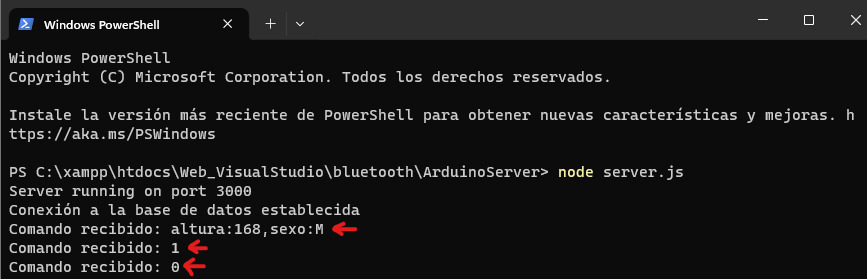
\includegraphics[width=1\textwidth]{img/C2_PruebasSistema/cmd.png}
    \caption{Terminal CMD muestra los datos recibidos por el servidor.}
    \label{fig:cmd}
\end{figure}

Por otro lado, el terminal de VS Code permitirá comprobar qué información se comparte entre Arduino y el servidor web. Si el funcionamiento es correcto se mostrarán por pantalla las acciones `realizar actividad' (Figura \ref{fig:realizarActividad}) e  `iniciar actividad' (Figura \ref{fig:iniciarActividad}) de forma similar a como sucedía en el terminal CMD. Al realizar una actividad de monitorización de la marcha, Arduino envía los datos registrados y estos son inmediatamente redirigidos al servidor, como se refleja en la Figura \ref{fig:datosActividad}.

\begin{figure}[h]
    \centering
    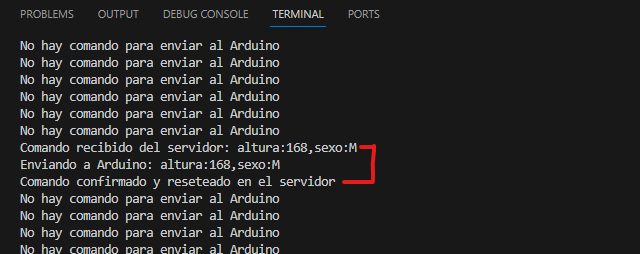
\includegraphics[width=1\textwidth]{img/C2_PruebasSistema/realizarActividad.png}
    \caption{Terminal VS Code. Acción `realizar actividad'.}
    \label{fig:realizarActividad}
\end{figure}

\begin{figure}[h]
    \centering
    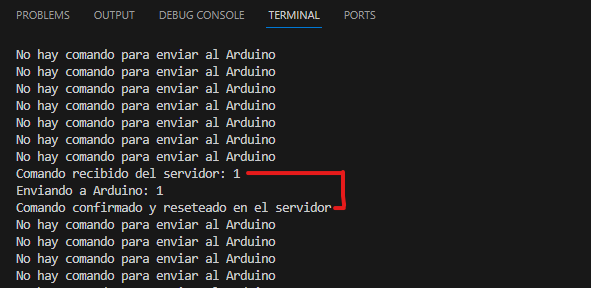
\includegraphics[width=1\textwidth]{img/C2_PruebasSistema/iniciarActividad.png}
    \caption{Terminal VS Code. Acción `iniciar actividad'.}
    \label{fig:iniciarActividad}
\end{figure}

\begin{figure}[h]
    \centering
    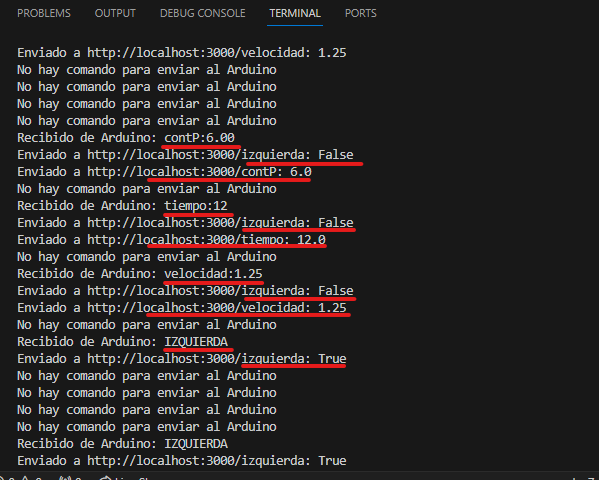
\includegraphics[width=1\textwidth]{img/C2_PruebasSistema/datosActividad.png}
    \caption{Terminal VS Code. Flujo de datos durante la realización de una actividad de marcha.}
    \label{fig:datosActividad}
\end{figure}


\section{Instrucciones para la modificación o mejora del proyecto.}

Este anexo comenta una serie de puntos que se deben tener en cuenta para continuar el desarrollo del proyecto software según se ha comentado en el apartado \textit{`Lineas de trabajo futuras'} de la memoria.

En cuanto a la realización de mejoras en la plataforma web, será imprescindible prestar atención a las siguientes áreas:
\begin{itemize}
    \item Implementar protocolos de seguridad avanzados como HTTPS, medidas de protección contra ataqes de inyección SQL y encriptado de contraseñas.
    \item Analizar la obtención de un diseño web que proporcione al usuario una experiencia más satisfactoria. Además, la plataforma desarrollada tiene un diseño responsivo que puede ser optimizado.
    \item Facilitar el acceso desde dispositivos externos migrando la web a un servidor en la nube. Al escoger el servidor se debe considerar la capacidad de escalabilidad que proporciona.
    \item Explorar la implementación de WebSockets para mejorar la comunicación en tiempo real. La plataforma actual implementa API REST como tecnología de comunicación.
    \item Complementar el sistema con el desarrollo de una aplicación móvil que funciona en paralelo con la plataforma web.
\end{itemize}

Respecto a las funcionalidades del sistema, sería interesante trabajar en las siguientes direcciones:
\begin{itemize}
    \item Incrementar el procesamiento de datos para obtener estadísticas más detalladas y útiles para su uso en el ámbito clínico.
    \item Registrar las fechas y horas de las actividades realizadas, así como los horarios de administración de la medicación, para evaluar con mayor precisión el efecto del tratamiento farmacológico en el paciente.
    \item Integrar en el software el proceso de calibración del sensor que registra los datos de la actividad, posibilitando al usuario resolver posibles problemas si dicho sensor comienza a presentar errores de lectura.
    \item Implementar una funcionalidad para el registro de datos de actividad sin conexión, permitiendo el almacenamiento posterior de datos en la base de datos. Esto podría lograrse añadiendo una tarjeta microSD en la que se almacena la información de forma temporal.
    \item Realizar la combinación con un sistema de control postural, como el desarrollado por \cite{NaiaraGa53:online}. El proyecto mencionado emplea las mismas herramientas que este, y requiere una conexión bluetooth, desarrollo de software y mejoras hardware, todo ello al mismo nivel que requería la versión previa de este proyecto. Esta integración estaría justificada por el objetivo de obtener un dispositivo de monitoreo integral de pacientes con EP que sea económicamente accesible.
\end{itemize}

 Los trabajos futuros de mejoras hardware pueden centrarse en los siguientes aspectos: 
\begin{itemize}
    \item Implementar un sistema de alerta eficaz para episodios de congelación de la marcha. Se podría considerar el uso de vibraciones o alarmas sonoras, y la adición de un laser que proyecte una referencia visual en el suelo para ayudar al paciente a superar la situación.
    \item Mejorar la precisión y fiabilidad en la lectura de datos del sensor MPU6050, mediante el uso del procesador digital de movimiento (DMP) integrado \cite{saragonz91:online}.
    \item Ampliar el sistema añadiendo un sensor MPU6050 para la pierna derecha \cite{saragonz91:online}.
    \item Realizar cambios para mejorar la portabilidad y comodidad del prototipo, aproximandolo a un dispositivo de uso cotidiano.
    \item Estudiar alternativas de microcontroladores con Bluetooth integrado, podría reducir el tamaño del hardware y mejorar el procesamiento.
\end{itemize}
